\documentclass{article}
\usepackage{graphicx}
\usepackage[hidelinks]{hyperref}
\usepackage[margin=1in]{geometry}
\usepackage{amsmath}

\title{Technical Handover: StomaML}
\author{Mia Lindblad, Valtteri Ahola, Markus Tarma, Soumyadipta Kar}
\date{March 2026}

\begin{document}

\maketitle
\tableofcontents
\newpage

\section{Overview}

This document covers how StomaML works, how to run it, and how it is put together under the hood. The scientific background and project motivation are covered in the final report, so they are not repeated here.

The handover is written with two audiences in mind. The first is end users or future project members who mainly need to run the application and understand what goes in and what comes out. The second is developers or maintainers who may need to debug things, redeploy, or build on top of the existing system. Because of this, the earlier sections focus on practical usage, while the later sections go into more technical detail about the software itself.

The source code is available at \href{https://github.com/valttteri/StomaML}{https://github.com/valttteri/StomaML}.

\section{Running the application}

\subsection{Recommended method: Docker Compose}

The simplest way to run StomaML locally is with Docker Compose. It starts both the frontend and backend at the same time and removes the need to set them up individually.

The file \texttt{docker-compose.yaml} in the repository defines the local multi-container setup. It currently includes two services:

\begin{itemize}
    \item \texttt{backend} -- built from \texttt{./backend} and exposed on port \texttt{8080}
    \item \texttt{frontend} -- built from \texttt{./frontend} and exposed on port \texttt{8050}
\end{itemize}

The frontend service also receives the environment variable

\begin{center}
\texttt{API\_URL=http://backend:8080/predict}
\end{center}

which lets the frontend container reach the backend through Docker Compose's internal networking. In other words, the frontend does not talk to \texttt{localhost} when running inside Compose -- it uses the service name \texttt{backend} instead.

To use this method, you need:
\begin{itemize}
    \item the full project repository,
    \item Docker and Docker Compose installed,
    \item the trained model weights placed at \texttt{backend/models/weights.pt}.
\end{itemize}

Open a terminal in the directory containing \texttt{docker-compose.yaml} and run:

\begin{center}
\texttt{docker compose up --build}
\end{center}

Docker will then build separate images for the frontend and backend using their respective \texttt{Dockerfile}s. Once everything is up, the frontend should be reachable at:

\begin{center}
\texttt{http://127.0.0.1:8050}
\end{center}

Docker might also show \texttt{0.0.0.0:8050} in its output, but for opening the app in a browser, \texttt{http://127.0.0.1:8050} or \texttt{http://localhost:8050} is usually the safest bet.

Once the interface loads in the browser, the application is ready. When done, press \texttt{Ctrl+C} in the same terminal to stop the containers.

Figure~\ref{fig:docker-compose} shows what a typical successful startup looks like.

\begin{figure}[h!]
    \centering
    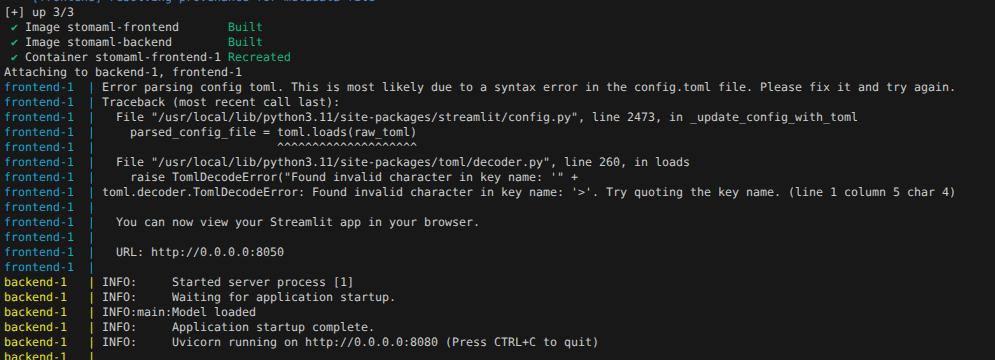
\includegraphics[width=1\linewidth]{Screenshot from 2026-03-10 20-47-00.png}
    \caption{Example of a successful Docker Compose startup. Some warning messages may appear but they do not prevent local use. The frontend URL is shown in the terminal output.}
    \label{fig:docker-compose}
\end{figure}

\subsubsection{In case of failure}

Some files are sensitive to line endings. A \texttt{.gitattributes} file is included to keep the repository on LF endings, but in practice shell scripts can still end up with CRLF on some systems or editors -- especially right after cloning.

If you see something like:

\begin{center}
\texttt{frontend-1 | exec /entrypoint.sh: no such file or directory}
\end{center}

the most likely cause is that \texttt{frontend/entrypoint.sh} has been saved with CRLF instead of LF.

In Visual Studio Code, you can fix this by opening the file, finding the \texttt{CRLF} indicator in the lower right corner, switching it to \texttt{LF}, and saving. Sometimes the editor needs a restart for the change to fully take effect.

\clearpage
\begin{figure}[h!]
    \centering
    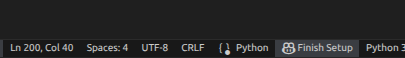
\includegraphics[width=0.5\linewidth]{Screenshot from 2026-03-11 10-26-13.png}
    \caption{The CRLF indicator in the lower right corner of Visual Studio Code.}
    \label{fig:button}
\end{figure}

If a container does not start, checking its logs is a good first step:

\begin{center}
\texttt{docker compose logs frontend}
\end{center}

or

\begin{center}
\texttt{docker compose logs backend}
\end{center}

You can also run:

\begin{center}
\texttt{docker compose ps}
\end{center}

This shows whether containers are running, which ports are mapped, and whether something exited right after starting.

Another common issue is port conflicts. If something else is already using one of the mapped ports, startup will fail. The ports used in this project are:

\begin{itemize}
    \item \texttt{8080} for the backend
    \item \texttt{8050} for the frontend
\end{itemize}

Either stop whatever is using the port, or change the port mapping in \texttt{docker-compose.yaml}.

\subsection{Running without Docker}

If Docker Compose is not an option, the frontend and backend can be run separately in local Python environments. This is more suited for development or troubleshooting than everyday use.

It is a good idea to use separate virtual environments for the frontend and backend so that their dependencies stay isolated. You can create one with:

\begin{center}
\texttt{python -m venv .venv}
\end{center}

After creating it, activate the environment before installing anything. The activation command depends on your OS and terminal.

\subsubsection{Backend}

To start the backend, open a terminal, go to the backend directory, remember to activate the virtual environment, install the dependencies, and launch the FastAPI app:

\begin{center}
\texttt{cd backend}
\end{center}

\begin{center}
\texttt{pip install -r requirements.txt}
\end{center}

\begin{center}
\texttt{uvicorn main:app --reload --host 0.0.0.0 --port 8000}
\end{center}

Make sure the model weights file exists at:

\begin{center}
\texttt{backend/models/weights.pt}
\end{center}

If the backend starts correctly, you can check its health endpoint at:

\begin{center}
\texttt{http://127.0.0.1:8000/health}
\end{center}

Note that the Dockerised backend uses port \texttt{8080}, while the example above uses \texttt{8000}. This is fine, but keep it in mind when debugging connectivity issues.
\subsubsection{Frontend}

Start the frontend in a second terminal (remember to activate the frontend virtual environment):

\begin{center}
\texttt{cd frontend}
\end{center}

\begin{center}
\texttt{pip install -r requirements.txt}
\end{center}

\begin{center}
\texttt{streamlit run main.py}
\end{center}

Before launching, make sure the frontend's configuration points to the right backend endpoint. For local development, that usually means setting \texttt{API\_URL} to:

\begin{center}
\texttt{http://127.0.0.1:8000/predict}
\end{center}

The \texttt{/predict} part matters -- the frontend sends requests directly to the prediction endpoint, not just the backend root URL. The confidence threshold and image scale are also passed along as query parameters in the request URL, for example:

\begin{center}
\texttt{http://127.0.0.1:8000/predict?conf=0.5\&scale=0.2174}
\end{center}

These are added automatically by the frontend when it sends a request, so there is no need to set them manually, but it is good to know they are part of the call when debugging.

When running things this way, the backend has to be up before the frontend can talk to it. If either service tries to use a port that is already taken, it will not start until the conflict is resolved.

\section{Output fields and calculations}\label{section:output_fields_and_calculations}

After processing, the application returns results for each uploaded image. These include summary values like stomata count and density measurements, as well as more detailed per-detection information. This section is particularly useful for end users, since it explains what each value in the CSV and JSON metadata files means and how it is computed. It is also relevant for future developers, because the calculation logic needs to stay consistent over time.

The backend returns one result object per uploaded image. Each result contains image-level information and a list of per-stomata metadata entries.

\subsection{Image-level summary output}

The \texttt{density\_info} object contains the following fields:

\begin{itemize}
    \item \texttt{total\_pixels} -- the total number of pixels in the image, calculated as:
    \[
    \texttt{image height} \times \texttt{image width}
    \]

    \item \texttt{non\_countable\_pixels} -- the number of pixels belonging to the union of all masks classified as non-countable area. In the current implementation, any detection whose class name is listed in \texttt{NON\_COUNTABLE\_CLASSES} contributes to this mask.

    \item \texttt{countable\_pixels} -- the number of pixels not covered by the non-countable mask. Simply the total pixels minus the non-countable ones.

    \item \texttt{stomata\_count} -- the number of detected stomata that made it into the final metadata list. In practice, this is just the length of the \texttt{stomata} list.

    \item \texttt{stomatal\_density\_per\_px2} -- stomatal density in stomata per pixel squared:
    \[
    \frac{\texttt{stomata\_count}}{\texttt{countable\_pixels}}
    \]
    If \texttt{countable\_pixels} is zero, this field is set to zero to avoid division by zero.

    \item \texttt{um\_per\_px} -- the image scale in micrometers per pixel, as provided by the user.

    \item \texttt{stomatal\_density\_per\_mm2} -- stomatal density converted to stomata per square millimetre. The conversion works by first turning the countable pixel area into mm\textsuperscript{2} using the image scale, and then dividing the stomata count by that area:
    \[
    \text{countable area in mm}^2 = \texttt{countable\_pixels} \times \left(\frac{\texttt{um\_per\_px}}{1000}\right)^2
    \]
    \[
    \texttt{stomatal\_density\_per\_mm2} = \frac{\texttt{stomata\_count}}{\text{countable area in mm}^2}
    \]
\end{itemize}

\subsection{Stomata-level metadata output}

Each detected stomata that passes filtering gets its own metadata dictionary. The fields are:

\begin{itemize}
    \item \texttt{id} -- a running index for the stomata within the image.

    \item \texttt{confidence} -- the model's predicted confidence for this detection.

    \item \texttt{pixel\_area} -- the number of pixels in the stomata's binary mask.

    \item \texttt{area\_um2} -- the mask area converted to square micrometers:
    \[
    \texttt{pixel\_area} \times \texttt{um\_per\_px}^2
    \]

    \item \texttt{bbox\_xyxy} -- the tight bounding box around the mask, given as $[x_{\min}, y_{\min}, x_{\max}, y_{\max}]$.

    \item \texttt{width\_px} and \texttt{height\_px} -- bounding box width and height in pixels.

    \item \texttt{centroid\_x} and \texttt{centroid\_y} -- the mean of all mask pixel coordinates.

    \item \texttt{length\_major\_axis\_px} and \texttt{length\_minor\_axis\_px} -- estimated from an ellipse fitted to the mask using OpenCV's \texttt{cv2.fitEllipse}. If the mask has fewer than five points, ellipse fitting is not possible and these values are \texttt{None}.

    \item \texttt{length\_major\_axis\_um} -- the major axis length converted to micrometers.

    \item \texttt{fraction\_in\_countable\_area} -- the fraction of the stomata mask that falls within countable area:
    \[
    \frac{\text{stomata mask pixels inside countable area}}{\texttt{pixel\_area}}
    \]
    A stomata is only kept if this value is at least 0.5.

    \item \texttt{closest\_stomata\_distance\_px}, \texttt{closest\_stomata\_distance\_um}, and \texttt{closest\_stomata\_distance\_mm} -- the Euclidean distance from this stomata's centroid to the nearest other stomata's centroid, in pixels, micrometers, and millimetres respectively. If there is only one stomata in the image, these are \texttt{None}.
\end{itemize}

\subsection{Processing order}

To understand the output, it helps to know the order of operations:

\begin{itemize}
    \item Detected stomata masks are first collected as candidates.
    \item Each candidate is checked against the countable region. Only those with at least 50\% of their area inside countable area become final metadata entries.
    \item Nearest-neighbour distances are calculated after all entries have been finalised, using centroid-to-centroid Euclidean distance.
    \item If the model returns no masks at all, the backend returns an empty stomata list and an empty \texttt{density\_info} dictionary.
\end{itemize}

\section{System structure}

StomaML has two main parts: a Streamlit frontend and a FastAPI backend. The frontend provides the user interface, handles file uploads, and shows results. The backend holds the machine learning model and all the inference logic.

In practice, the user only interacts with the frontend. When an analysis is started, the frontend sends the uploaded files and chosen parameters to the backend API. The backend loads the trained model, runs segmentation, turns the detections into structured output, and sends everything back for the frontend to display and offer for download.

This split keeps the interface simple for end users while letting the ML and API logic live in their own maintainable part of the codebase.

\section{Repository structure}

The repository mirrors this division. \texttt{frontend/} contains the Streamlit application, and \texttt{backend/} contains the FastAPI service and inference logic. Trained model weights go in \texttt{backend/models/weights.pt}. The \texttt{docker-compose.yaml} at the root defines the local multi-container setup, and each service has its own \texttt{Dockerfile} for containerised deployment.

This layout makes it easy to work on the UI and the model-serving logic independently.

\section{Frontend}

\subsection{Role of the frontend}

The frontend is the part of the application that users actually see. It is built with Streamlit so that everything can be done in a browser rather than on the command line. Its job is intentionally narrow: collect user input, send requests to the backend, and present the results. It does not do any machine learning computation.

This separation matters for maintenance. The frontend handles interaction and presentation only. All model loading, inference, post-processing, and scientific calculations live in the backend. So if you need to change the analysis logic, do it in the backend. If you need to change how things look or what the user sees, do it in the frontend.

\subsection{Frontend files}

The frontend code lives in \texttt{frontend/}. The main files are:

\begin{itemize}
    \item \texttt{main.py} -- the main Streamlit application. It defines the UI, handles file upload, sends inference requests to the backend, tracks progress, and renders the results and download buttons.
    \item \texttt{config.py} -- loads the backend API URL from the \texttt{API\_URL} environment variable, keeping deployment-specific addresses out of the main application code.
    \item \texttt{utils.py} -- small helper classes: a wrapper around Streamlit's progress bar and a utility for estimating remaining processing time during batch inference.
    \item \texttt{requirements.txt} -- Python dependencies for the frontend.
    \item \texttt{Dockerfile} -- defines the container image build for the frontend.
    \item \texttt{entrypoint.sh} -- the container startup script. It sets up a Streamlit configuration directory and then launches the application.
\end{itemize}

There is also a Streamlit configuration file at \texttt{.streamlit/config.toml}, discussed further in the Streamlit configuration subsection below.

\subsection{Frontend behaviour}

The frontend is a straightforward single-page application. The workflow goes like this:

\begin{enumerate}
    \item The user uploads one or more image files.
    \item The user sets two numerical values: image scale and confidence threshold.
    \item The user presses the analysis button.
    \item The frontend sends the images and parameters to the backend.
    \item The frontend receives the JSON response, pulls out the image-level and stomata-level results, and shows the summary in a table.
    \item The user can download the summary as a CSV and the per-stomata metadata as a JSON file.
\end{enumerate}

Accepted file types are \texttt{jpg}, \texttt{jpeg}, and \texttt{png}. Multiple files can be uploaded and processed in one go. The details of how batch processing works are described in the batch processing subsection below.

\subsection{User inputs in the frontend}

Besides the uploaded files, the interface exposes two numeric parameters.

\paragraph{Image scale}
The image scale is entered as micrometers per pixel. The default value is:
\[
\frac{10}{46} \approx 0.2174
\]
This comes from the project's default calibration assumption that $10\,\mu\text{m}$ corresponds to 46 pixels. The help text in the UI communicates this to the user. The value is passed unchanged to the backend, which uses it to convert pixel-based measurements into physical units.

\paragraph{Confidence threshold}
The confidence threshold defaults to 0.5, with an accepted range of 0.01 to 0.99 in the frontend. It is sent to the backend as the \texttt{conf} query parameter and controls which detections the model pipeline keeps.

\subsection{Implementation details of \texttt{main.py}}

The main UI logic lives in \texttt{frontend/main.py}. It has three helper functions and one main application function.

\paragraph{\texttt{call\_api\_with\_files}}
Handles communication with the backend. It takes a list of file paths along with the confidence threshold and image scale, packs the files into a multipart request via \texttt{requests.post()}, and sends the numeric settings as request parameters. The backend address comes from \texttt{API\_URL} (imported from \texttt{config.py}).

The request timeout is currently set to 120 seconds. If a request fails, the exception is shown to the user through Streamlit and then re-raised. This means errors are not silently swallowed, which is helpful for debugging but may look somewhat technical to non-developer users.

\paragraph{\texttt{download\_csv}}
Takes a Pandas DataFrame with the image-level results and creates a Streamlit download button. The file is exported as UTF-8 CSV under the name \texttt{stoma\_results.csv}. The DataFrame index is included in the output.

\paragraph{\texttt{download\_metadata}}
Converts per-stomata metadata into formatted JSON and offers it as a download. The output file is called \texttt{metadata.json}. This is meant for anyone who needs more detail than what the summary table shows.

\paragraph{\texttt{main}}
The \texttt{main()} function defines the page itself. It sets the title, initialises session state, renders the upload widget and input fields, handles the reset button, runs the analysis when requested, and then shows the results table and download buttons.

Two session state variables are used:

\begin{itemize}
    \item \texttt{inference\_done} -- a boolean flag for whether processing has finished and results should be shown.
    \item \texttt{file\_uploader} -- an integer key used to reset the file uploader widget. Incrementing it forces Streamlit to recreate the widget, which clears the selected files.
\end{itemize}

This reset trick is a common Streamlit pattern and is worth keeping if the upload logic gets changed later.

\subsection{Layout and interaction design}

The frontend uses a compact layout built from Streamlit columns and standard widgets. After uploading files, the page shows:

\begin{itemize}
    \item a numeric input for image scale,
    \item a numeric input for confidence threshold,
    \item a metric showing how many files are uploaded,
    \item a reset button for clearing the uploads,
    \item a button for starting analysis.
\end{itemize}

While the analysis runs, two dynamic elements are displayed:

\begin{itemize}
    \item a text status showing that analysis is in progress with an estimated time remaining,
    \item a progress bar that updates after each processed file.
\end{itemize}

After processing finishes, the page shows a results table under the heading \texttt{Analysis results}, followed by download buttons for CSV and JSON output.

The layout is kept simple on purpose. Future groups could certainly improve it, but the current design gets the basic workflow across clearly enough.

\subsection{Batch processing behaviour}

Even though multiple files can be uploaded at once, the frontend does not send them all in a single request. It loops through the files and sends them one at a time. For each image:

\begin{enumerate}
    \item the uploaded file is written to a temporary file,
    \item the temp file path is passed to the API request helper,
    \item the backend response is read,
    \item image-level and stomata-level data are appended to result arrays,
    \item the progress bar and time estimate are updated.
\end{enumerate}

This keeps the frontend logic simple and makes progress tracking straightforward, since each completed image maps directly to one progress update. The downside is that total runtime may be longer than a more advanced batching approach would give, especially with many files.

\subsection{Displayed results}

After all files have been processed, the frontend builds a Pandas DataFrame using the \texttt{density\_info} fields described in Section~\ref{section:output_fields_and_calculations}. A \texttt{Filename} column is added and used as the index, so each row corresponds to one image. The table is rendered with \texttt{st.dataframe(..., use\_container\_width=True)} to fill the available page width.

Only image-level summary values are shown directly on the page. The more detailed per-stomata records are only available in the downloaded JSON metadata file.

\subsection{Progress bar and remaining time estimation}

The file \texttt{frontend/utils.py} has two small utility classes.

\paragraph{\texttt{ProgressBar}}
A thin wrapper around Streamlit's built-in progress bar. It keeps track of the current value and width, and exposes \texttt{render()} for initial display and \texttt{update()} for changing the value during processing. It is not a complex component -- just a small abstraction to keep the main code tidier.

\paragraph{\texttt{RemainingTime}}
Estimates how much time is left during multi-file inference. It tracks the total file count, the number already processed, and a queue of recent processing times. The logic works as follows:

\begin{itemize}
    \item for the first few files, it just shows \texttt{...} instead of a number,
    \item it stores up to the 15 most recent inference times,
    \item it averages those times,
    \item it multiplies the average by the number of remaining files,
    \item it formats the result as minutes and seconds.
\end{itemize}

This is a rough estimate meant purely as a usability convenience. It has no effect on the actual inference.

\subsection{Configuration handling}

As mentioned in the frontend files overview, backend connectivity is configured through \texttt{frontend/config.py}, which reads:

\begin{center}
\texttt{API\_URL = os.getenv("API\_URL")}
\end{center}

The backend address differs between local development, Docker Compose, and OpenShift, so keeping it in an environment variable rather than hardcoded is important. If \texttt{API\_URL} is missing or wrong, requests will fail as soon as the user tries to run an analysis.

\subsection{Containerisation and startup}

The frontend has its own \texttt{Dockerfile}. The container image is currently built from \texttt{python:3.11}. The build process:

\begin{enumerate}
    \item sets \texttt{/frontend} as the working directory,
    \item copies \texttt{requirements.txt} and installs dependencies,
    \item copies the frontend source files into the image,
    \item copies \texttt{entrypoint.sh} to the container root,
    \item makes the entrypoint script executable,
    \item exposes port 8050,
    \item runs the entrypoint script on container start.
\end{enumerate}

The startup script \texttt{entrypoint.sh} does a bit of setup before launching Streamlit. It creates a temporary configuration directory at \texttt{/tmp/.streamlit}, writes a minimal \texttt{config.toml} that turns off usage statistics, sets \texttt{HOME} and \texttt{STREAMLIT\_CONFIG\_DIR} accordingly, and then launches:

\begin{center}
\texttt{streamlit run main.py --server.address 0.0.0.0 --server.port "\$\{PORT:-8050\}"}
\end{center}

The \texttt{\$\{PORT:-8050\}} bit means the container defaults to port 8050 but can adapt if a hosting platform injects a different port via the \texttt{PORT} variable.

\subsection{Streamlit configuration}

The project includes a Streamlit configuration file at \texttt{.streamlit/config.toml}. It has browser and server settings. Telemetry is disabled with:

\begin{center}
\texttt{gatherUsageStats = false}
\end{center}

and CORS is enabled with an explicit list of allowed origins, covering both local development and deployed URLs. This matters because the frontend may not work properly if requests come from a host that Streamlit does not recognise.

One thing to be aware of is that there are currently two related configuration mechanisms:

\begin{itemize}
    \item the project-level \texttt{.streamlit/config.toml}, and
    \item the runtime configuration generated inside the container by \texttt{entrypoint.sh}.
\end{itemize}

Right now, the entrypoint-generated config only writes the telemetry setting and does not include the CORS origin list from the repository-level file. So Streamlit behaviour might differ slightly depending on whether you run the app from source or through the container.

\subsection{Dependencies}

The frontend dependencies in \texttt{frontend/requirements.txt} are:

\begin{itemize}
    \item \texttt{streamlit==1.53.1}
    \item \texttt{python-dotenv}
    \item \texttt{streamlit-ext==0.1.19}
\end{itemize}

The most important one is Streamlit itself, since it provides the entire UI layer.

\subsection{Maintenance considerations}

Most frontend work in the future will probably happen in \texttt{frontend/main.py}. Typical changes might include:

\begin{itemize}
    \item adjusting layout and visuals,
    \item improving status messages and error reporting,
    \item adding input validation or clearer user guidance,
    \item supporting additional result visualisations,
    \item previewing uploaded images or processed outputs,
    \item better handling of large file batches.
\end{itemize}

A few implementation details are worth understanding before changing anything:

\begin{itemize}
    \item The file uploader reset works by changing the Streamlit widget key through session state.
    \item The displayed results depend on the backend returning \texttt{density\_info} fields in an order consistent with the DataFrame column list.
    \item Backend communication relies entirely on \texttt{API\_URL} being correct.
    \item The progress display assumes files are processed sequentially, one request per image.
\end{itemize}

For anyone maintaining the frontend, the good news is that the logic is compact and mostly linear. The key thing to remember is that it is a presentation layer only. Any changes to scientific calculations, segmentation behaviour, mask interpretation, or returned metadata should go in the backend.

\section{Backend}

\subsection{Role of the backend}

The backend is the computational core of StomaML. It takes uploaded images from the frontend, loads the trained segmentation model, runs inference, computes derived measurements, and returns everything as structured JSON. In short, the backend is where all the scientifically relevant computation happens.

Its job can be broken down into four steps. First, it loads the trained YOLO segmentation model at startup. Second, it exposes API endpoints through FastAPI so the frontend can send requests. Third, it runs inference on uploaded microscope images and post-processes the segmentation results into structured measurements. Fourth, it returns only the fields that the frontend and downloadable outputs actually need. This keeps the frontend lightweight and the analysis logic in one place.

\subsection{Backend files}

The backend code lives in \texttt{backend/}. The main files are:

\begin{itemize}
    \item \texttt{main.py} -- defines the FastAPI application, sets up middleware, loads the model at startup, and exposes the API endpoints.
    \item \texttt{utils/inference.py} -- the inference and post-processing pipeline. This file turns raw YOLO outputs into the JSON-compatible result structure that the API returns.
    \item \texttt{utils/model\_utils.py} -- the \texttt{ModelManager} class, responsible for loading the model once and reusing it across requests.
    \item \texttt{models/weights.pt} -- the trained model weights needed at runtime.
    \item \texttt{requirements.txt} -- backend Python dependencies.
    \item \texttt{Dockerfile} -- the backend container image definition for local and deployed use.
\end{itemize}

The division of work is simple: \texttt{main.py} handles the application lifecycle and HTTP layer, \texttt{model\_utils.py} handles model access, and \texttt{inference.py} handles image processing and measurement logic.

\subsection{FastAPI application structure}

The backend is defined in \texttt{backend/main.py}. It uses FastAPI with a lifespan function to make sure the model gets loaded during startup rather than on the first prediction request.

Logging is set to \texttt{INFO} level. A global \texttt{ModelManager} instance is created at import time, and the lifespan function then calls:

\begin{center}
\texttt{model\_manager.load\_model("models/weights.pt")}
\end{center}

If this fails, the backend does not start at all. This is intentional -- it makes problems like missing files or incompatible weights show up immediately rather than only when someone tries to run their first analysis.

The FastAPI app is created with the title \texttt{Stoma Segmentation API}. It also uses trusted host middleware to restrict which host headers it accepts.

\subsection{Trusted host middleware}

The backend adds \texttt{TrustedHostMiddleware} with a specific list of allowed hosts. Currently that list includes:

\begin{itemize}
    \item \texttt{stoma-ml-api-stoma-ml.apps.ocp-test-0.k8s.it.helsinki.fi}
    \item \texttt{stoma-ml-api-stoma-ml.apps.ocp-bm-0.k8s.it.helsinki.fi}
    \item \texttt{localhost}
    \item \texttt{127.0.0.1}
    \item \texttt{backend}
\end{itemize}

This is especially relevant for deployment. If the backend ever gets exposed under a new hostname and that hostname is not added here, requests will be rejected even if the service itself is running fine. So this is one of the first things to update after any hostname change.

\subsection{API endpoints}

The backend has three endpoints.

\paragraph{\texttt{GET /}}
Returns a simple status message:
\begin{center}
\texttt{\{"status": "healthy", "message": "Stoma Segmentation API is running"\}}
\end{center}
It is mainly there as a quick check that the service is up.

\paragraph{\texttt{GET /health}}
Returns:
\begin{center}
\texttt{\{"status": "healthy", "model\_loaded": ...\}}
\end{center}
where \texttt{model\_loaded} is a boolean from \texttt{model\_manager.is\_loaded()}. More informative than the root endpoint, because it tells you not just that the process is running, but also whether the model loaded successfully.

\paragraph{\texttt{POST /predict}}
The main inference endpoint. It accepts:

\begin{itemize}
    \item one or more uploaded files via \texttt{files: List[UploadFile]},
    \item a confidence threshold via the query parameter \texttt{conf},
    \item an image scale via the query parameter \texttt{scale}.
\end{itemize}

Parameter validation in FastAPI:
\begin{itemize}
    \item \texttt{conf}: default 0.25, range $0.0 \leq \texttt{conf} \leq 1.0$,
    \item \texttt{scale}: default $10/46$, must be strictly greater than 0.
\end{itemize}

Before running inference, the endpoint checks a few things:

\begin{itemize}
    \item if the model is not loaded, it returns HTTP 503,
    \item if no files were provided, it returns HTTP 400,
    \item if all uploaded files are empty, it returns HTTP 400.
\end{itemize}

It then reads the file contents into memory, stores them as \texttt{(filename, bytes)} tuples, calls the batch inference pipeline, and returns a cleaned response containing only the fields meant for downstream use.

\subsection{Returned API response structure}

The \texttt{/predict} endpoint returns JSON with this top-level structure:

\begin{center}
\texttt{\{"total\_images": ..., "results": [...]\}}
\end{center}

Each entry in \texttt{results} contains:

\begin{itemize}
    \item \texttt{filename}
    \item \texttt{index}
    \item \texttt{success}
    \item \texttt{density\_info}
    \item \texttt{stomata}
\end{itemize}

This explicit cleaning step in \texttt{main.py} prevents accidental leakage of internal fields if the inference code changes later. The frontend depends only on this cleaned format, not on every internal detail of the processing pipeline.

\subsection{Model manager}

Model loading is wrapped in the \texttt{ModelManager} class in \texttt{utils/model\_utils.py}. It provides a small abstraction over the underlying \texttt{YOLO} model object.

It contains:

\begin{itemize}
    \item a private lock (\texttt{\_lock}),
    \item a private model reference (\texttt{\_model}),
    \item \texttt{load\_model(weights\_path)},
    \item \texttt{is\_loaded()},
    \item \texttt{get\_model()}.
\end{itemize}

The lock makes model initialisation thread-safe. The main purpose of the class is to guarantee the model is loaded once and then reused for all subsequent requests. This avoids repeated model construction and keeps route handlers simple.

For future maintainers: route functions should not create YOLO models directly. Always go through the manager.

\subsection{Inference pipeline}

The core inference logic is in \texttt{utils/inference.py}. At a high level, the pipeline does the following:

\begin{enumerate}
    \item raw uploaded image bytes are decoded into an RGB image using Pillow,
    \item the image is passed to the YOLO segmentation model,
    \item the prediction result is post-processed into binary masks and metadata,
    \item stomata-level records and image-level density statistics are computed,
    \item the result is returned as a JSON-compatible Python dictionary.
\end{enumerate}

The YOLO model is called with:
\begin{center}
\texttt{model(image, conf=conf\_threshold, imgsz=640, retina\_masks=True, rect=False, iou=0.25)[0]}
\end{center}

So inference currently uses image size 640, retina-quality masks, no rectangular inference, and an IoU threshold of 0.25. If model or deployment requirements change down the line, these are among the most likely parameters to revisit.

\subsection{Mask handling and post-processing}

The raw YOLO segmentation output is not returned as-is. Instead, \texttt{process\_detections()} transforms it into a more stable, application-specific structure.

For each predicted mask, the pipeline:

\begin{itemize}
    \item retrieves the floating-point mask array,
    \item retrieves the associated confidence and predicted class,
    \item thresholds the mask at 0.5 to get a binary mask,
    \item resizes it to the original image dimensions if needed (nearest-neighbour interpolation),
    \item checks whether the class is non-countable,
    \item if non-countable, merges the mask into the global non-countable mask,
    \item if the class is \texttt{stomata}, stores it as a candidate for further filtering.
\end{itemize}

The non-countable classes are currently:

\begin{center}
\texttt{NON\_COUNTABLE\_CLASSES = \{"nothing", "trichome", "vein"\}}
\end{center}

After the global non-countable mask is built, the countable region is defined as every pixel not covered by it. Each stomata candidate is then checked: it is only included in the final results if at least

\begin{center}
\texttt{COUNTABLE\_OVERLAP\_THRESHOLD = 0.5}
\end{center}

of its mask area lies within countable area. Candidates that overlap too much with non-countable regions get excluded from the stomata list and therefore also from density calculations.

This is an important point for maintenance. If a future model uses different class names, or if the definition of countable area changes, both \texttt{NON\_COUNTABLE\_CLASSES} and the overlap threshold may need updating. Otherwise the reported counts and densities might not match the intended biological interpretation.

\subsection{Image-level calculations}

After all masks are processed, the backend computes an image-level summary called \texttt{density\_info}, containing the fields described in Section~\ref{section:output_fields_and_calculations}. These are derived from the original image dimensions, the union of non-countable masks, the number of accepted stomata, and the user-provided scale. Density in mm\textsuperscript{2} is computed by the helper \texttt{density\_per\_mm2()}, which converts the countable pixel area to square millimetres and then divides stomata count by that area.

\subsection{Stomata-level calculations}

For each accepted stomata, the backend creates a metadata dictionary using \texttt{build\_metadata()}, containing the per-stomata fields described in Section~\ref{section:output_fields_and_calculations}. The implementation details worth highlighting here are:

\begin{itemize}
    \item Stomata length is estimated by fitting an ellipse to the binary mask via OpenCV's \texttt{cv2.fitEllipse}. The major axis is used as the length estimate. If the mask has fewer than five points, ellipse fitting cannot be done and the length values are \texttt{None}. This is an approximation, not a direct biological measurement.
    \item Nearest-neighbour distances are computed by \texttt{add\_closest\_stomata\_distance()} after all metadata entries have been created. These are centroid-to-centroid Euclidean distances, not edge-to-edge. If only one stomata is present, the distance fields are \texttt{None}.
    \item The \texttt{fraction\_in\_countable\_area} field serves a dual purpose: it is both a diagnostic value and a record of why a particular stomata was included.
\end{itemize}

\subsection{Functions in \texttt{utils/inference.py}}

The main helper functions in the inference module are:

\begin{itemize}
    \item \texttt{mask\_to\_bbox()} -- computes a tight bounding box around a binary mask.
    \item \texttt{get\_ellipse\_length()} -- fits an ellipse to mask pixels and returns the major and minor axis lengths.
    \item \texttt{build\_metadata()} -- creates one per-stomata metadata dictionary.
    \item \texttt{add\_closest\_stomata\_distance()} -- computes nearest-neighbour distances across all stomata in an image.
    \item \texttt{density\_per\_mm2()} -- converts countable area to mm\textsuperscript{2} and computes density.
    \item \texttt{process\_detections()} -- transforms one raw YOLO result into stomata metadata and density summary, builds the non-countable mask, and filters stomata candidates by their overlap with countable area.
    \item \texttt{run\_inference()} -- end-to-end inference for a single image.
    \item \texttt{batch\_inference()} -- loops over a list of uploaded images and calls \texttt{run\_inference()} on each.
\end{itemize}

Despite the name \texttt{batch\_inference}, the implementation is sequential: images are processed one after another in a loop. This matches the frontend, which also sends files one at a time.

\subsection{Error handling}

The API-level error codes (HTTP 503 for missing model, HTTP 400 for missing or empty files) were already described in the API endpoints subsection. Beyond that, \texttt{run\_inference()} wraps the processing in a \texttt{try}/\texttt{except} block, logs the exception, and re-raises it. So inference errors show up in backend logs rather than being silently ignored.

In practice, debugging usually involves checking container or server logs when the frontend only reports that a request failed. That is expected -- the backend logs are where the useful details are.

\subsection{Runtime defaults and constants}

The two key constants \texttt{NON\_COUNTABLE\_CLASSES} and \texttt{COUNTABLE\_OVERLAP\_THRESHOLD} were already introduced in the mask handling subsection above. Having them as named constants makes it fairly easy to adapt the backend if a future model uses different class labels or if the overlap rule needs changing.

\subsection{Dependencies}

Backend dependencies are in \texttt{backend/requirements.txt}. The main ones are:

\begin{itemize}
    \item \texttt{fastapi==0.128.2}
    \item \texttt{uvicorn==0.40.0}
    \item \texttt{python-multipart}
    \item \texttt{pillow}
    \item \texttt{numpy}
    \item \texttt{ultralytics==8.4.12}
    \item \texttt{opencv-python-headless}
\end{itemize}

The Docker image also explicitly installs CPU-only PyTorch and Torchvision before the rest of the dependencies. This matters because \texttt{ultralytics} depends on PyTorch, and the container is set up for CPU inference rather than GPU.

Any major upgrade to \texttt{ultralytics}, \texttt{torch}, or \texttt{opencv} should be tested carefully since it could affect model loading, output format, or mask handling.

\subsection{Containerisation}

The backend has its own \texttt{Dockerfile}, built from \texttt{python:3.10-slim}. The build process:

\begin{enumerate}
    \item sets \texttt{/app} as the working directory,
    \item installs system libraries needed by the model stack and OpenCV,
    \item copies \texttt{requirements.txt},
    \item installs CPU-only PyTorch and Torchvision from the PyTorch CPU wheel index,
    \item installs the Python dependencies from \texttt{requirements.txt},
    \item copies \texttt{main.py},
    \item copies the \texttt{utils/} directory,
    \item creates a \texttt{models/} directory and copies \texttt{models/weights.pt},
    \item exposes port 8080,
    \item starts Uvicorn on port 8080.
\end{enumerate}

\subsection{Maintenance considerations}

Most backend work in the future will likely be in \texttt{backend/main.py} and especially \texttt{backend/utils/inference.py}. Common tasks might include:

\begin{itemize}
    \item updating the model weights,
    \item adapting to changed class names or mappings,
    \item changing post-processing logic,
    \item adding new output fields,
    \item improving validation and error reporting,
    \item optimising inference performance,
    \item introducing automated tests for output consistency.
\end{itemize}

A few key assumptions to keep in mind (most already discussed in the subsections above):

\begin{itemize}
    \item The backend assumes YOLO mask outputs can be thresholded at 0.5 and treated as binary segmentation masks.
    \item The distinction between stomata and non-countable area depends entirely on the class names the model predicts.
    \item The frontend expects the response to contain \texttt{density\_info} and \texttt{stomata} fields with specific names.
\end{itemize}

Since the backend is the scientific core, even small logic changes here can alter the reported biological measurements. Any such change should be documented and tested end-to-end with the frontend.


\section{Deployment}

\subsection{OpenShift}

The deployed version runs on OpenShift in containers. The frontend and backend are separate services, each with its own container image and runtime configuration. Communication between them depends on correct routing and environment settings.

This section documents the application-specific deployment assumptions for running StomaML on OpenShift. It is not a guide to OpenShift platform administration in general.

From the application's perspective, the key deployment facts are:

\begin{itemize}
    \item the frontend and backend are deployed separately,
    \item the frontend needs the correct backend prediction endpoint,
    \item the backend needs access to the model weights file at runtime,
    \item hostname-related backend settings must match the deployed route.
\end{itemize}

One important detail: the frontend gets the backend URL as a secret. Because the frontend code expects a full prediction endpoint, this value should point to the \texttt{/predict} route, not just the backend root URL.

On the backend side, the model weights must be available at runtime. The expected path inside the backend project is:

\begin{center}
\texttt{models/weights.pt}
\end{center}

Without this file, the backend will fail at startup since the model is loaded when FastAPI starts.

Also remember that the backend uses trusted host middleware. If the backend route hostname changes, the allowed host list has to be updated too. Otherwise requests get rejected even though the service is running.

A practical way to think about deployment is that three things all need to be right at the same time:

\begin{enumerate}
    \item the containers start successfully,
    \item the frontend points to the correct backend endpoint,
    \item the backend accepts requests for the deployed hostname and has access to the model weights.
\end{enumerate}

If any one of these is off, the deployment will look broken even if the other parts work fine.

\subsection{Local use and testing}

Although OpenShift is the main deployment target, local execution is still important for development, testing, and debugging. The essentials are the same: backend dependencies installed, model weights present, backend starts, and the frontend points to the right endpoint.

For most people, Docker Compose is the easiest option because it avoids the manual setup of running two services separately. The local Compose setup is also useful because it mirrors the deployed architecture reasonably well -- frontend and backend still run as separate services talking over HTTP.

\section{Checks after changes}

After any meaningful change, it is a good idea to run a short end-to-end test. This goes for both code changes and deployment changes, since configuration issues often only show up when you exercise the full system.

A minimal check should include:

\begin{enumerate}
    \item confirm that the backend starts successfully,
    \item verify that the backend health endpoint responds,
    \item launch the frontend,
    \item verify that the frontend can reach the backend,
    \item run a test analysis on one or more sample images,
    \item confirm that the results table and downloadable files look reasonable.
\end{enumerate}

For local development, that typically means checking the health endpoint first and then opening the frontend in a browser. For OpenShift, it means verifying both the frontend and backend routes, then doing at least one real analysis through the frontend.

The most likely failure points after deployment changes are:

\begin{itemize}
    \item wrong backend URL in the frontend configuration,
    \item missing or inaccessible model weights,
    \item hostname changes not reflected in trusted host settings,
    \item services starting successfully but without actual end-to-end connectivity.
\end{itemize}

A deployment should not be considered done just because the containers are running. At least one full analysis should be tested after meaningful changes.

\end{document}